\begin{block}{Conceptual Framework}
    \begin{figure}
        \caption{NASA images of the Ohio-Mississippi system (L) April 2010; (R) May 2011}
        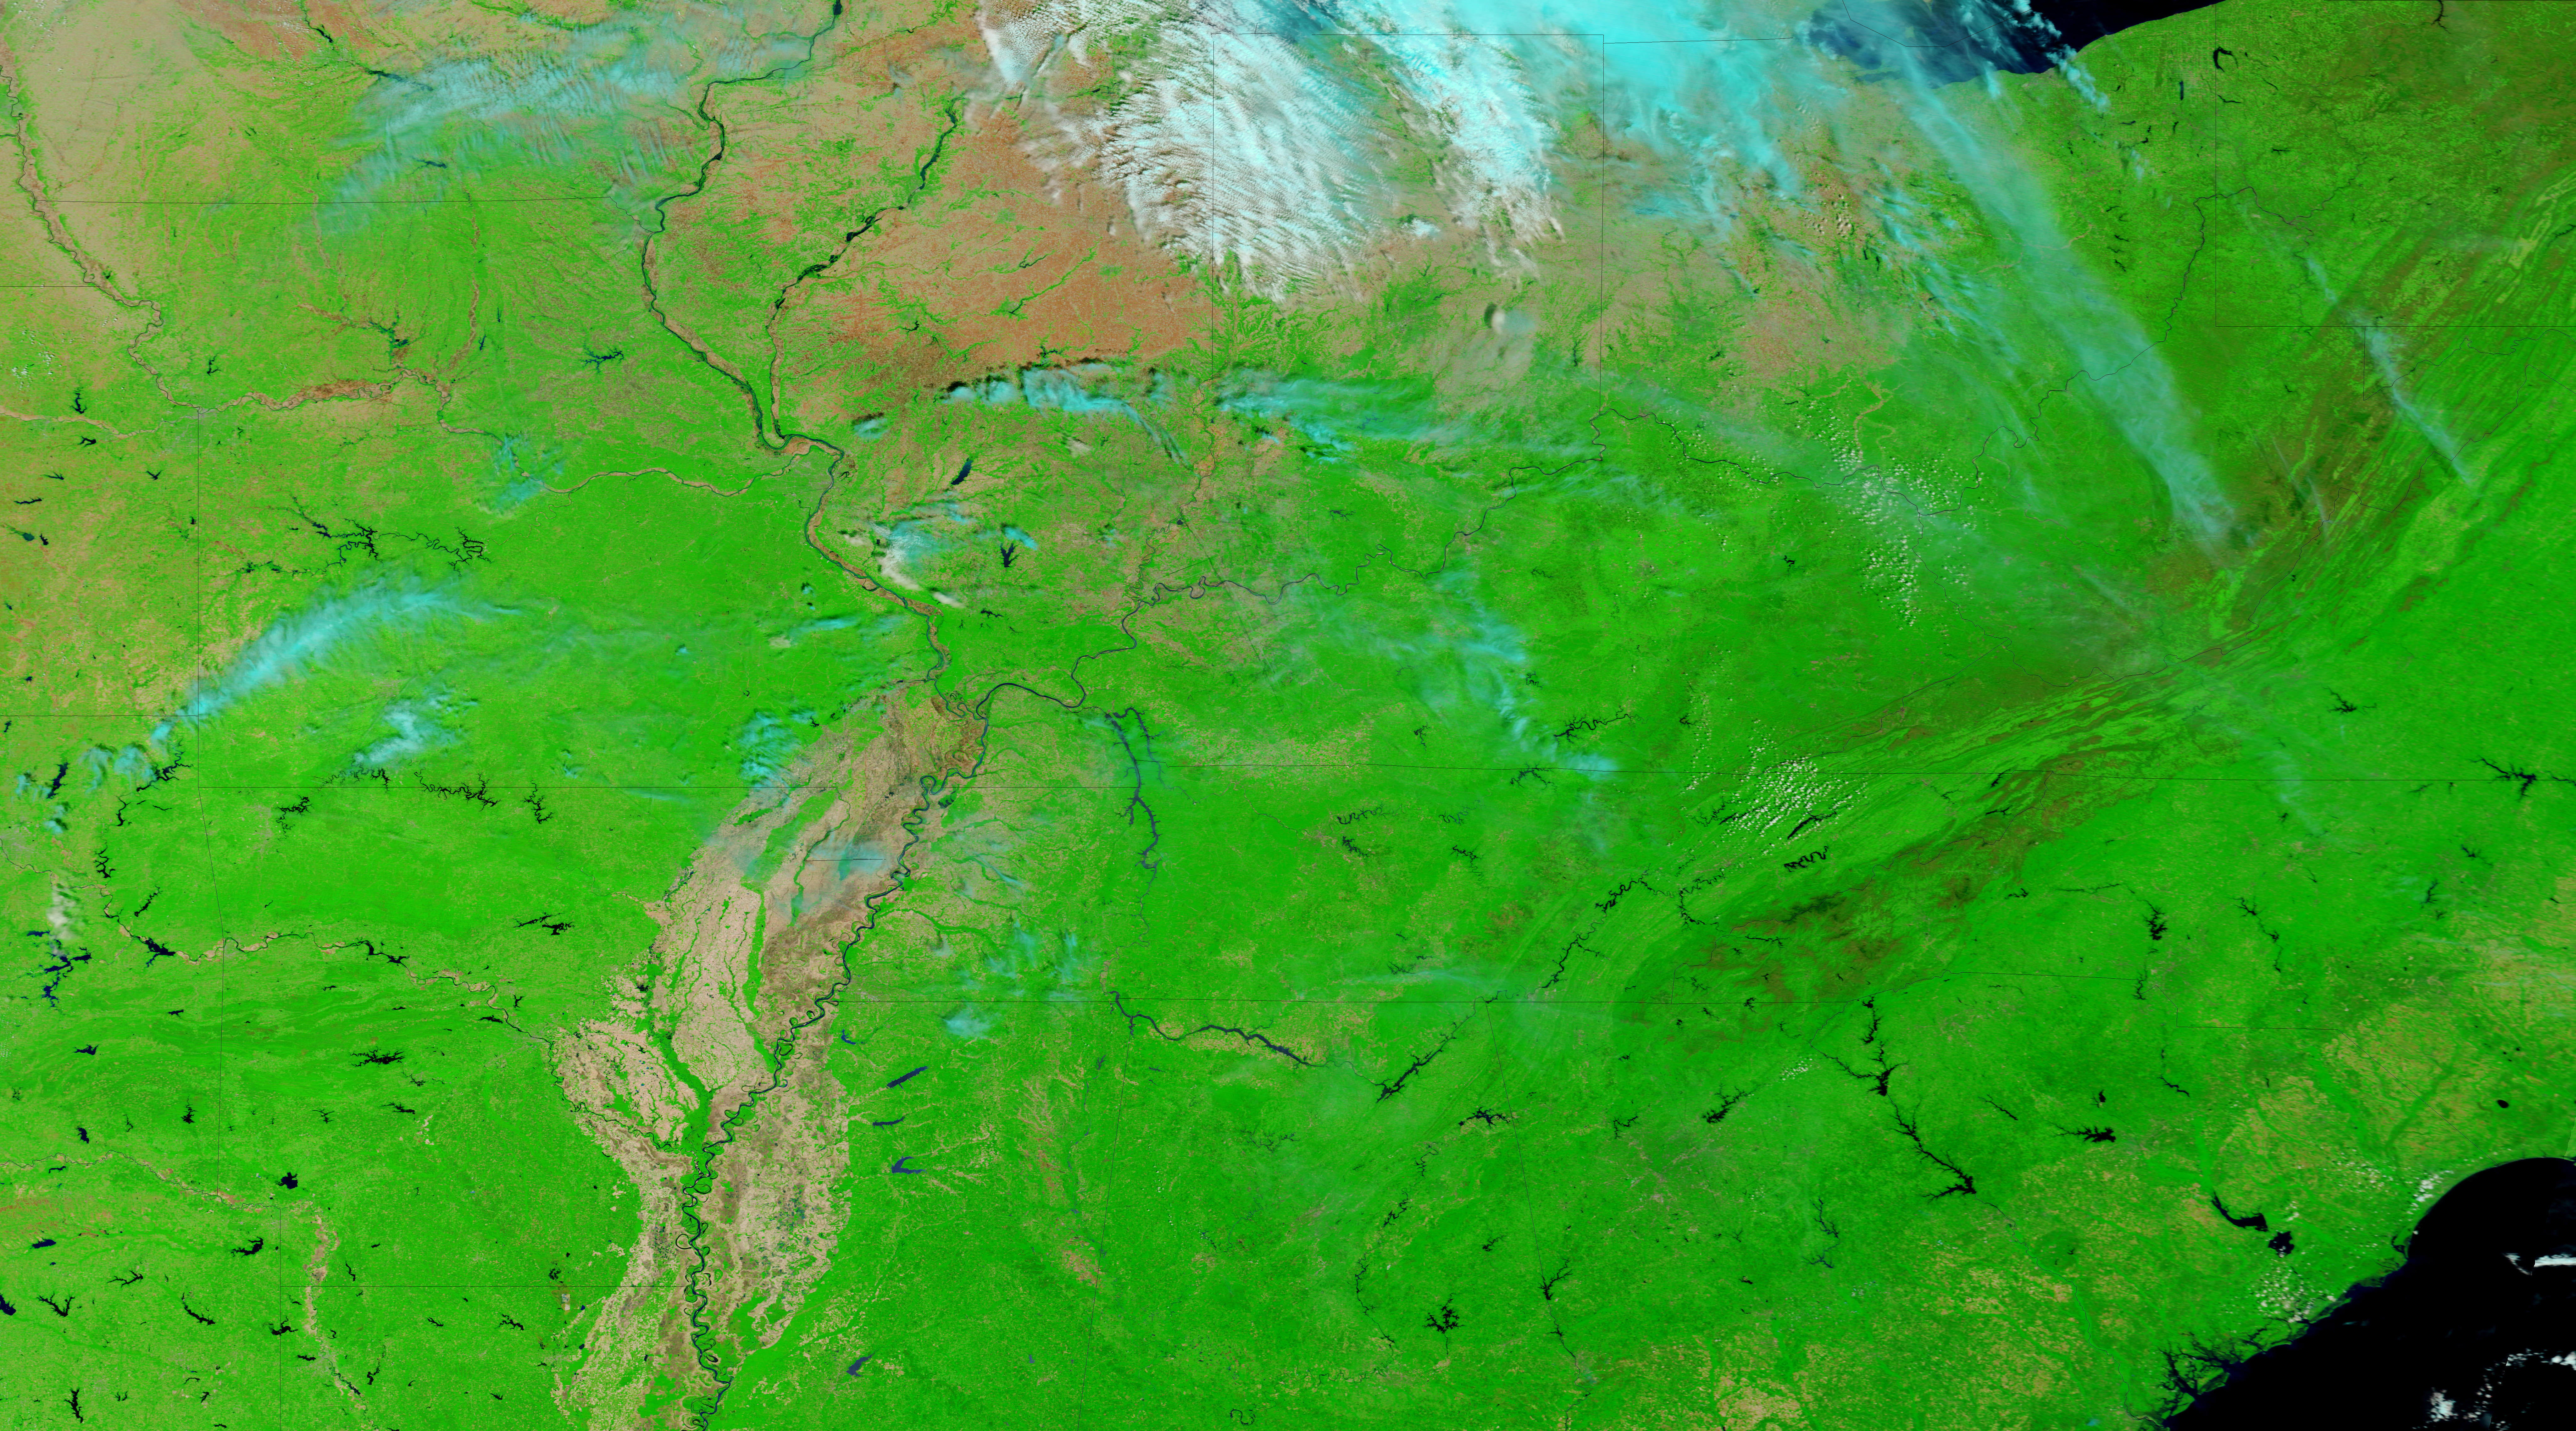
\includegraphics[width=0.475\columnwidth]{../FigExternal/nasa_april_2010}~
        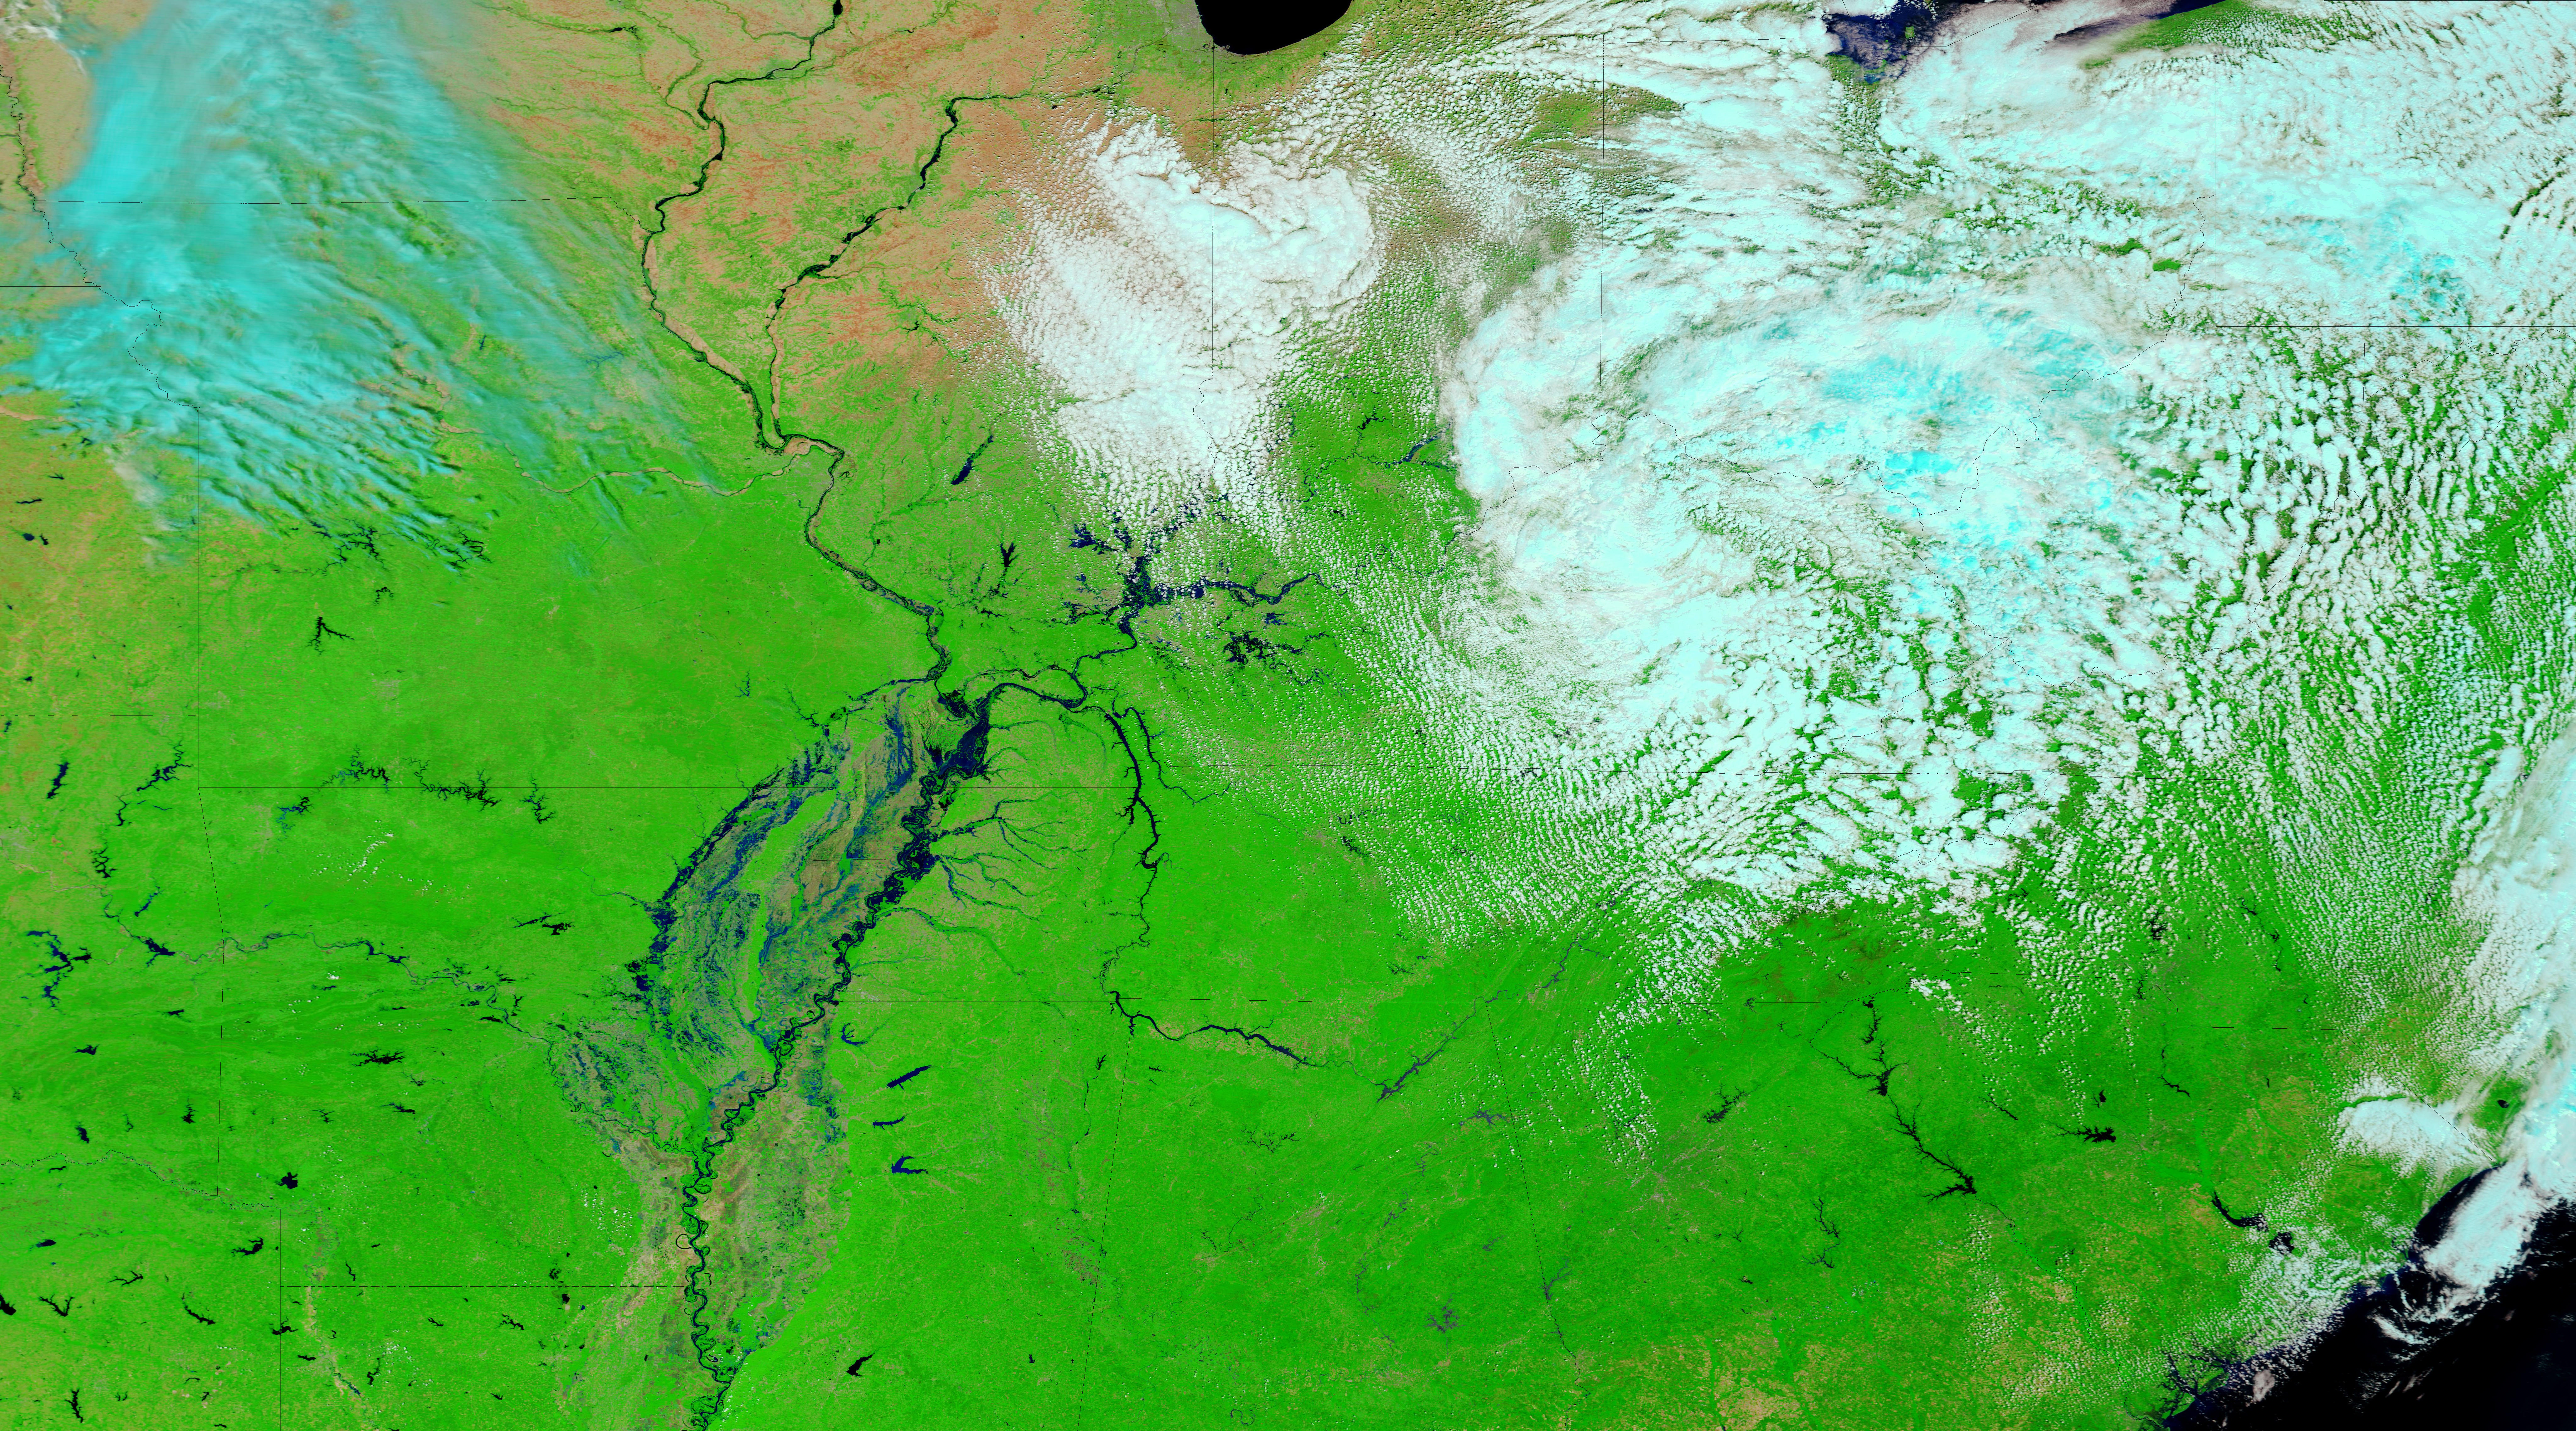
\includegraphics[width=0.475\columnwidth]{../FigExternal/nasa_may_2011}
        \label{fig:nasa-2010-11}
    \end{figure}
    Credible forecasting of flood probabilities at sub-seasonal to decadal timescales \cite{Merz2014} requires understanding the \textbf{cross-timescale dynamics that regulate the the large-scale transport \& convergence of moisture}: specific circulations mechanisms which are modulated by global-scale circulations and persistent, low-frequency boundary conditions.
    For example, the April 2011 flooding in the Ohio-Mississippi river system (\cref{fig:apr2011,fig:nasa-2010-11}) was driven by steering of consecutive storm systems to the region.
    \begin{figure}
        \begin{tikzpicture}[node distance = 1.15cm, auto, font=\sffamily]
	% Place nodes
	\node [action] (boundary) {Boundary Forcings};
	\node [object, below= of boundary] (circulation) {Circulation Anomaly};
	\node [object, below=of circulation] (steering) {Moisture Steering};
	\node [action, below= of steering] (flood) {High Flood Potential};
	% Draw edges
	\path [arrow] (boundary) -- (circulation);
    \path [arrow] (circulation) -- (steering);
    \path [arrow] (steering) -- (flood);
\end{tikzpicture}
~\hfill
        \includegraphics[width=0.5\columnwidth]{flooding_2011_flooding}
        \caption{(L) Conceptual diagram. (R) Tracked cyclones (lines) and strongest 20\% monthly-mean \SI{250}{\hecto\pascal} winds for April 2011. Region affected circled in blue.}
        \label{fig:apr2011}
    \end{figure}
\end{block}
